\documentclass[12pt, a4paper, oneside]{report}

% Required Packages
\usepackage[a4paper, margin=1in]{geometry}
\usepackage{graphicx}
\usepackage{setspace}
\usepackage{titlesec}
\usepackage{fancyhdr}
\usepackage{hyperref}
\usepackage{booktabs}
\usepackage{longtable}
\usepackage{array}
\usepackage[table]{xcolor}
\usepackage{listings}
\usepackage{enumitem}
\usepackage{caption}
\usepackage{subcaption}
\usepackage{tocloft}
\usepackage[T1]{fontenc}
\usepackage[utf8]{inputenc}
\usepackage{microtype}
\usepackage{parskip}
\usepackage{amsmath}
\usepackage{float}
\usepackage{tabularx}
\usepackage{multirow}
\usepackage{cite}
\usepackage{tikz}
\usetikzlibrary{shapes.geometric, arrows.meta, positioning, fit, backgrounds, calc}
\usepackage[many]{tcolorbox}

% Brand Colors
\definecolor{brandteal}{RGB}{0, 77, 64}
\definecolor{brandblue}{RGB}{0, 175, 254}
\definecolor{darkgray}{RGB}{50, 50, 50}
\definecolor{lightgray}{RGB}{245, 245, 245}
\definecolor{codegreen}{RGB}{0, 128, 0}
\definecolor{codegray}{RGB}{128, 128, 128}
\definecolor{codered}{RGB}{180, 0, 0}

% Code Listing Style
\lstset{
  backgroundcolor=\color{lightgray},
  basicstyle=\ttfamily\small,
  keywordstyle=\color{brandteal}\bfseries,
  commentstyle=\color{codegreen}\itshape,
  stringstyle=\color{codered},
  numberstyle=\tiny\color{codegray},
  numbers=left,
  numbersep=5pt,
  frame=single,
  framerule=0.4pt,
  rulecolor=\color{brandteal},
  breaklines=true,
  captionpos=b,
  tabsize=2
}

% Page Layout & Headers
\pagestyle{fancy}
\fancyhf{}
\fancyhead[L]{\textbf{\textcolor{brandteal}{Pather Saathi}}}
\renewcommand{\chaptermark}[1]{\markboth{\thechapter.\ #1}{}}
\fancyhead[R]{\textbf{\textcolor{darkgray}{\small\leftmark}}}
\fancyfoot[C]{\textbf{\thepage}}
\renewcommand{\headrulewidth}{0.4pt}
\renewcommand{\headrule}{\hbox to\headwidth{\color{brandteal}\leaders\hrule height \headrulewidth\hfill}}
\setlength{\headheight}{24.64995pt}

% Title Formatting
\titleformat{\chapter}[display]
  {\normalfont\huge\bfseries\color{brandteal}}
  {\Large\textsc{\chaptertitlename}\ \thechapter}
  {1ex}
  {\Huge}[\vspace{1ex}\color{brandteal}\titlerule]
\titleformat{\section}
  {\normalfont\Large\bfseries\color{darkgray}}
  {\thesection}{1em}{}
\titleformat{\subsection}
  {\normalfont\normalsize\bfseries\color{brandteal}}
  {\thesubsection}{1em}{}

% Custom TColorBox Environments
\newtcolorbox{engineeringnote}[1][]{
  enhanced, colback=lightgray, colframe=brandteal, coltitle=white,
  title=\textbf{Engineering Note}, fonttitle=\bfseries,
  attach boxed title to top left={yshift=-2mm, xshift=5mm},
  boxed title style={sharp corners},
  arc=0mm, top=3mm, bottom=3mm, left=3mm, right=3mm, #1
}
\newtcolorbox{keyfinding}[1][]{
  enhanced, colback=white, colframe=brandblue, coltitle=white,
  title=\textbf{Key Finding}, fonttitle=\bfseries,
  attach boxed title to top left={yshift=-2mm, xshift=5mm},
  boxed title style={sharp corners},
  arc=0mm, top=3mm, bottom=3mm, left=3mm, right=3mm, #1
}
\newtcolorbox{lessonslearned}[1][]{
  enhanced, colback=white, colframe=codered, coltitle=white,
  title=\textbf{Lesson Learned}, fonttitle=\bfseries,
  attach boxed title to top left={yshift=-2mm, xshift=5mm},
  boxed title style={sharp corners},
  arc=0mm, top=3mm, bottom=3mm, left=3mm, right=3mm, #1
}

% Screenshot Macro
\newcommand{\screenshot}[3]{
  \begin{figure}[H]
      \centering
      \begin{tcolorbox}[enhanced, colback=lightgray!20, colframe=darkgray, boxrule=0.5pt, arc=2mm, width=0.85\textwidth]
          \centering
          #1
      \end{tcolorbox}
      \caption{#2}
      \label{fig:#3}
  \end{figure}
}



% Spacing
\setstretch{1.5}
\setlength{\parskip}{6pt}

\begin{document}

% --- TITLE PAGE ---
\begin{titlepage}
    \begin{tikzpicture}[remember picture, overlay]
        % Background geometric shapes for a modern startup whitepaper feel
        \fill[brandteal] (current page.north west) rectangle ($(current page.north east)+(0,-3)$);
        \fill[lightgray] (current page.south west) rectangle ($(current page.south east)+(0,3)$);
    \end{tikzpicture}

    \vspace*{-2cm}
    \begin{center}
        \textcolor{white}{\LARGE \textbf{BARAK VALLEY ENGINEERING COLLEGE}}\\[0.2cm]
        \textcolor{white}{\large Department of Computer Science and Engineering}\\[0.2cm]
        \textcolor{white}{\large Assam Science and Technology University (ASTU)}
    \end{center}

    \vspace{3cm}

    \begin{center}
        
\includegraphics[width=5cm]{logo.png}\\[1.5cm] % Keep logo size
        {\Huge \textbf{\textcolor{brandteal}{PATHER SAATHI}}}\\[0.5cm]
        {\LARGE \textbf{\textcolor{darkgray}{A Fleet Booking Platform for Barak Valley}}}\\[0.8cm]
        
        \begin{tcolorbox}[enhanced, colback=white, colframe=brandteal, arc=0mm, boxrule=1pt, width=0.8\textwidth, center]
            \centering \textit{\Large AI-Augmented Development $\times$ Local Impact}
        \end{tcolorbox}
    \end{center}

    \vfill
    
    \begin{center}
        {\large A Project Report submitted in partial fulfillment of the requirements for the degree of}\\[0.3cm]
        {\Large \textbf{Bachelor of Technology in Computer Science and Engineering}}\\[1.5cm]
    \end{center}
    
    \begin{minipage}[t]{0.45\textwidth}
        \begin{flushleft}
            \textbf{\textcolor{brandteal}{Submitted by:}}\\
            \vspace{0.2cm}
            \textbf{Biswajyoti Nath}\\
            \textbf{Dipjyoti Roy}\\
            \textbf{Subinoy Nath}\\
        \end{flushleft}
    \end{minipage}
    \hfill
    \begin{minipage}[t]{0.45\textwidth}
        \begin{flushright}
            \textbf{\textcolor{brandteal}{Under the guidance of:}}\\
            \vspace{0.2cm}
            \textbf{Khanjan Changmai Baruah}\\
            \relax Assistant Professor\\
        \end{flushright}
    \end{minipage}
    
    \vspace{1.5cm}
    \begin{center}
        \textbf{\textcolor{darkgray}{Academic Year: 2025--2026}}
    \end{center}
    \vspace*{1cm}
\end{titlepage}

% --- CERTIFICATE PAGE ---
\newpage
\thispagestyle{empty}
\begin{center}
    {\Huge \textbf{CERTIFICATE}}\par
    \vspace{1.5cm}
\end{center}

\begin{spacing}{1.5}
This is to certify that the project entitled \textbf{"PATHER SAATHI --- A Fleet Booking Platform for Barak Valley"} submitted by \textbf{Biswajyoti Nath, Dipjyoti Roy, and Subinoy Nath} in partial fulfillment of the requirements for the award of the degree of Bachelor of Technology in Computer Science and Engineering from \textbf{Assam Science and Technology University (ASTU)} is a bonafide record of the work carried out by them under my supervision.
\end{spacing}

\vspace{3cm}

\begin{flushright}
    \textbf{Khanjan Changmai Baruah}\\
    \relax Assistant Professor\\
    \vspace{1.5cm}
    \textbf{Dr. Kausthav Pratim Kalita}\\
    Head of Department\\
    \relax Assistant Professor
\end{flushright}

\vspace{1.5cm}
\noindent Date: June 2026\\
Place: Sribhumi

% --- DECLARATION PAGE ---
\newpage
\thispagestyle{empty}
\begin{center}
    {\Huge \textbf{DECLARATION}}\par
    \vspace{1.5cm}
\end{center}

\begin{spacing}{1.5}
We hereby declare that the project report entitled \textbf{"PATHER SAATHI --- A Fleet Booking Platform for Barak Valley"} submitted in partial fulfillment of the requirements for the degree of Bachelor of Technology in Computer Science and Engineering at \textbf{BARAK VALLEY ENGINEERING COLLEGE}, affiliated with \textbf{Assam Science and Technology University (ASTU)}, is an authentic record of our own original work carried out under the guidance of \textbf{Khanjan Changmai Baruah}.

We further declare that the work presented in this report has not been submitted previously, in part or in full, to any other university or institution for the award of any degree or diploma. All sources of information and references have been duly acknowledged.
\end{spacing}

\vspace{3cm}

\begin{flushright}
    \textbf{Biswajyoti Nath}\\
    \vspace{1cm}
    \textbf{Dipjyoti Roy}\\
    \vspace{1cm}
    \textbf{Subinoy Nath}
\end{flushright}

\vspace{1.5cm}
\noindent Date: June 2026\\
Place: Sribhumi

% --- ACKNOWLEDGEMENT PAGE ---
\newpage
\thispagestyle{empty}
\begin{center}
    {\Huge \textbf{ACKNOWLEDGEMENT}}\par
    \vspace{1.5cm}
\end{center}

\begin{spacing}{1.5}
We would like to express our deepest gratitude to our project guide, \textbf{Mr. Khanjan Changmai Baruah}, whose expert guidance, continuous encouragement, and insightful feedback have been instrumental in the successful completion of this project. Their deep understanding of software engineering and commitment to rigorous methodology shaped the architectural direction of Pather Saathi.

We extend our sincere thanks to our Head of Department, \textbf{Dr. Kausthav Pratim Kalita}, for providing us with the necessary resources, academic environment, and institutional support required to undertake this intensive research and development endeavour.

We are profoundly grateful to \textbf{BARAK VALLEY ENGINEERING COLLEGE} for fostering an environment of innovation and technical excellence that enabled this work.

A special note of acknowledgement goes to the local fleet operators in Barak Valley, specifically those operating the Silchar-Hailakandi route, who generously participated in our field surveys. Their firsthand insights into the daily operational challenges of manual fleet management provided the foundational requirements for this platform.

Finally, we acknowledge the transformative impact of open-source tools and AI platforms in our development workflow. The integration of Next.js, Supabase, and Vercel, alongside the orchestration of AI models via the Model Context Protocol (MCP), fundamentally empowered us to deliver an enterprise-grade solution within the constraints of a student project.
\end{spacing}

% --- ABSTRACT PAGE ---
\newpage
\thispagestyle{empty}
\begin{center}
    {\Huge \textbf{ABSTRACT}}\par
    \vspace{1.5cm}
\end{center}

\begin{spacing}{1.5}
Inter-district transportation in Tier-3 Indian regions, specifically Barak Valley, Assam, relies heavily on analogue, highly fragmented coordination methods. Fleet operators manage bookings via physical ledgers and phone calls, leading to pervasive double bookings and unutilised capacity. Customers, conversely, lack any digital discovery mechanism to query available routes or secure seat reservations, resulting in significant friction. \textit{Pather Saathi} resolves this gap by providing an ultra-localised, cloud-native fleet booking platform tailored to the constraints of regional demographics. 

The platform implements atomic booking allocation using robust PostgreSQL Row Level Security (RLS) policies and Role-Based Access Control (RBAC), completely eliminating concurrency issues. Unlike metropolitan solutions that force proprietary app adoption, Pather Saathi adopts a WhatsApp-first interaction model, leveraging deep-linking to route booking confirmations and operator communications through the universally adopted messenger layer.

Methodologically, this project validates a multi-model AI-augmented development pipeline. Using the Model Context Protocol (MCP), AI agents were orchestrated to accelerate implementation while the human engineering team focused on architectural design and rigorous adversarial security audits. The final product was successfully deployed using a serverless architecture (Vercel and Supabase), achieving a highly scalable production environment with minimal monthly infrastructural cost. The result is a financially viable, enterprise-grade solution poised to democratise digital fleet management in underserved regions.

\vspace{1cm}
\textbf{Keywords:} Fleet Booking, Barak Valley, Serverless Architecture, Row Level Security, AI-Augmented Development, Model Context Protocol, WhatsApp Integration.
\end{spacing}

% --- TOC, LOF, LOT ---
\newpage
\pagenumbering{roman}
\renewcommand{\cftchapfont}{\bfseries\color{darkgray}}
\renewcommand{\cftchappagefont}{\bfseries\color{brandteal}}
\renewcommand{\cftsecfont}{\normalfont\color{darkgray}}
\renewcommand{\cftchapleader}{\cftdotfill{\cftdotsep}}

\tableofcontents
\newpage
\listoffigures
\newpage
\listoftables
\newpage
\pagenumbering{arabic}

% --- CHAPTER 1 ---
\chapter{Introduction and Objectives}

\section{Background}
The digital transformation of transportation infrastructure represents one of the most critical catalysts for economic mobility in developing regions. In Tier 3 Indian geographies, particularly in regions characterised by complex topographies and underdeveloped digital ecosystems, the gap between available technology and local adoption remains historically significant. While metropolitan areas benefit from highly integrated mobility-as-a-service (MaaS) applications that seamlessly connect passengers with transit networks, rural and semi-urban districts continue to rely on informal, analogue methods for transit coordination. The infrastructural context in Northeast India, and particularly Barak Valley, is uniquely challenging. The terrain and historical underinvestment have made inter-district road transport the primary artery for civilian mobility. Despite high smartphone penetration and ubiquitous Jio 4G internet access, the local transport sector remains technologically isolated.

\section{About the Project}
``Pather Saathi'' is a specialised, web-based fleet booking platform engineered precisely for the socioeconomic and technological realities of Barak Valley. The platform serves two primary user cohorts: local fleet operators who manage inter-district travel, and the passengers who rely on these services. Geographically, the project targets the crucial transit corridors connecting Silchar, Hailakandi, and Karimganj (Sribhumi). By leveraging low-friction communication channels like WhatsApp for confirmations, alongside a robust progressive web application interface, the platform digitises the booking lifecycle. It enables customers to discover available routes, view pricing, and request seats, while providing operators with a cloud-based dashboard to manage their fleet, approve bookings, and eliminate manual ledger errors.

\section{Objectives}
The primary objectives of this project are strictly defined and measurable:
\begin{enumerate}
    \item To design and implement a web-based fleet booking platform specifically tailored for Barak Valley operators and customers.
    \item To enable real-time seat availability tracking and atomic booking allocation to resolve the systemic issue of double bookings.
    \item To implement a secure, multi-tenant operator dashboard enforcing strict Role-Based Access Control (RBAC).
    \item To demonstrate and validate a multi-model AI-augmented development methodology leveraging Model Context Protocol (MCP) tooling.
    \item To deploy a production-grade system using serverless architecture that incurs zero initial infrastructure cost for local operators.
    \item To validate the system's security posture via rigorous adversarial testing of database policies prior to production deployment.
\end{enumerate}

\section{Key Contributions}
This report documents several key technical contributions to the field of localized software engineering:
\begin{itemize}[leftmargin=*]
    \item \textbf{Zero-Cost Architecture:} Architected a production-grade fleet management system with Rs 0/month fixed infrastructure costs using Vercel and Supabase.
    \item \textbf{WhatsApp Deep-Link Protocol:} Designed a seamless, no-API-cost booking confirmation flow utilizing \texttt{wa.me} dynamic URI generation.
    \item \textbf{Atomic Seat Allocation:} Implemented strict PostgreSQL transactions and Row Level Security to mathematically prevent double bookings.
    \item \textbf{AI-Augmented Methodology:} Pioneered a multi-model development pipeline utilizing MCP, significantly increasing engineering velocity for small teams.
    \item \textbf{Tier 3 UX Optimizations:} Built an extremely lightweight SSR frontend tailored specifically for mid-range Android devices on variable 4G connections.
\end{itemize}

\section{Report Organisation}
This report is organised to systematically document the engineering lifecycle of Pather Saathi. Chapter 2 defines the precise problem statement and existing pain points. Chapter 3 reviews current literature on transport digitisation and AI methodologies. Chapter 4 details the proposed solution and feature set. Chapter 5 outlines the AI-augmented agile methodology. Chapter 6 specifies system requirements. Chapter 7 dives deeply into the system architecture, database schema, and security model. Chapter 8 presents the results of adversarial testing and build verification. Chapter 9 discusses critical technical challenges encountered and resolved. Chapter 10 explores future scalability, and Chapter 11 provides the final conclusion.

% --- CHAPTER 2 ---
\chapter{Problem Statement}

\section{Current State of Fleet Booking in Barak Valley}
The current state of inter-district transport coordination in Barak Valley relies entirely on analogue and fragmented communication systems. Fleet bookings---whether for individual seats on scheduled bus routes or the chartering of whole vehicles for events---are executed predominantly through direct telephone calls, physical ledger entries, and ad-hoc WhatsApp messaging. Operators manage their daily inventory using pen-and-paper notebooks at physical transit hubs. Passengers seeking transportation must rely on personal connections or physical visits to transit stands to ascertain vehicle availability, departure times, and pricing. This reliance on synchronous, manual communication creates a high-friction environment that actively suppresses the economic potential of the local transport sector.

\section{Operator Pain Points}
For fleet operators, these manual processes manifest as severe operational pain points. The most critical issue is the high frequency of double bookings, which occurs when multiple requests are received simultaneously via phone and WhatsApp, leading to human error in ledger management. Operators also suffer from idle fleet capacity. Without a centralised digital broadcasting mechanism, vehicles frequently depart with unutilised seating, or whole vehicles sit idle in depots because potential customers are unaware of their availability. The lack of a unified dashboard means operators have zero real-time visibility into their projected revenue, fleet utilisation metrics, or driver assignments, preventing data-driven business optimisation.

\section{Customer Pain Points}
Conversely, the customers face significant friction when interacting with this analogue system. The primary pain point is the complete absence of a digital discovery mechanism. A customer cannot simply query available routes between Silchar and Hailakandi; they must already know which operator services that route and possess their contact information. Once a booking is verbally agreed upon, there is no formal digital confirmation, leading to anxiety and uncertainty. They completely lack any mechanism for tracking the status of their booking, requesting formal cancellations, or securely managing their travel itineraries. 

\section{Why Existing Solutions Fail}
While existing generic booking platforms and large-scale aggregators dominate metropolitan markets, they categorically fail to fit the context of Barak Valley. Enterprise-level solutions impose prohibitive subscription costs and require operators to possess advanced digital literacy and dedicated administrative staff. National aggregators extract significant commission percentages, which operates counter to the low-margin reality of local fleet owners. These generic platforms also attempt to force users into proprietary in-app messaging systems, ignoring the reality that WhatsApp is the universally accepted digital communication layer in this demographic. Furthermore, national systems like IRCTC cater exclusively to rail networks, offering no solutions for crucial intra-district road transport. 

\section{Formal Problem Statement}
The inter-district road transport sector in Barak Valley suffers from critical operational inefficiencies due to a reliance on fragmented, analogue booking methods (phone calls and paper ledgers), leading to high rates of double bookings, unutilised fleet capacity, and immense customer friction in discovering and securing transit options. There is an urgent need for an ultra-localised, low-cost digital fleet management platform that digitises discovery and guarantees atomic seat allocation while aligning with the region's existing digital literacy and reliance on WhatsApp communication.

% --- CHAPTER 3 ---
\chapter{Literature Survey}

\section{Digital Transformation of Transportation in India}
The digital transformation of transportation networks across India has historically been concentrated in Tier 1 and Tier 2 cities, driven by the rapid expansion of mobility-as-a-service (MaaS) platforms like Ola and Uber. Sharma and Das \cite{indicative1} comprehensively outline this metropolitan bias, noting that while urban centres benefit from sophisticated algorithmic dispatch and dynamic pricing models, rural and Tier 3 regions are systematically excluded due to lower anticipated profit margins and vastly different operational paradigms. Their research emphasises that digitising transport in these underserved areas requires bespoke, highly localised platforms that address specific regional constraints rather than attempting to retrofit heavy metropolitan architectures.

\section{Fleet Management Systems --- Existing Solutions}
A review of existing fleet management systems by Gupta \cite{indicative2} categorises modern solutions into two distinct verticals: high-end enterprise resource planning (ERP) integrations and consumer-facing aggregator platforms. Enterprise solutions, while feature-rich regarding telematics and predictive maintenance, impose prohibitive licensing costs and demand dedicated IT infrastructure, rendering them entirely unviable for small-scale regional operators in Barak Valley. Conversely, consumer aggregators operate on aggressive commission models that threaten the already narrow profit margins of local fleets. Gupta's analysis concludes that a significant market gap exists for lightweight, low-capital-expenditure management tools tailored for independent operators.

\section{Web Application Security for Booking Platforms}
Security in transactional web applications remains a critical focus area. The OWASP Top Ten \cite{owasp} provides a foundational framework for identifying systemic vulnerabilities, with Broken Access Control and Injection consistently ranking as primary threats. In the context of booking platforms, ensuring atomic transactions to prevent double bookings (a race condition exploit) is paramount. Literature dictates that security boundaries must be enforced at the database level using strict Row Level Security (RLS) rather than relying solely on application-layer logic, ensuring that tenant data remains perfectly isolated even in a multi-tenant cloud environment.

\section{AI-Augmented Software Development}
The most rapidly evolving domain in software engineering literature is the shift from manual coding to AI-orchestrated development. The introduction of the Model Context Protocol (MCP) by Anthropic has fundamentally altered the development paradigm, allowing Large Language Models (LLMs) to directly interface with local filesystems, version control, and database instances. Recent industry analyses indicate that multi-model workflows---where different AI agents are utilised for ideation, implementation, and adversarial review---produce software that rivals or exceeds the quality of traditional development teams \cite{indicative3}. This project serves as a practical validation of this emerging literature.

\section{UX Design for Tier 3 Indian Users}
Human-Computer Interaction (HCI) research focused on Tier 3 Indian demographics stresses the necessity of designing for constraint. Users in these demographics predominantly utilise mid-range Android devices on variable 4G networks, necessitating low-bandwidth optimisations and mobile-first responsive design. Literature on digital literacy in rural India indicates that adopting familiar interaction patterns---specifically those mimicking WhatsApp---drastically reduces the cognitive load required for user onboarding \cite{indicative4}.

\section{Summary and Research Gap}
The intersection of these literature domains reveals a distinct research gap. While AI methodologies are advancing rapidly, their application to solve hyper-localised, Tier-3 socio-economic problems remains sparse. Furthermore, existing transport platforms are economically and technologically unsuited for Barak Valley. Pather Saathi addresses this gap by applying cutting-edge AI-augmented development to engineer a secure, highly accessible, context-aware mobility solution.

\begin{table}[H]
    \centering
    \caption{Literature Survey Summary and Identified Gaps}
    \renewcommand{\arraystretch}{1.5}
    \begin{tabularx}{\textwidth}{l X X}
    \toprule
    \rowcolor{brandteal}
    \textcolor{white}{\textbf{Area}} & \textcolor{white}{\textbf{Existing Work}} & \textcolor{white}{\textbf{Gap Identified}} \\
    \midrule
    \rowcolor{lightgray}
    Transport Digitisation & Focused heavily on Tier 1/2 MaaS platforms. & Neglects intra-district road transport in Tier 3 regions. \\
    Fleet Management & High-cost ERPs or commission-heavy aggregators. & Lack of low-cost, lightweight tools for independent local operators. \\
    \rowcolor{lightgray}
    UX Design & Complex in-app proprietary messaging and heavy clients. & Failure to leverage universally adopted WhatsApp infrastructure. \\
    AI Development & Theoretical discussions on LLM coding capabilities. & Lack of end-to-end case studies using MCP for full-stack production apps. \\
    \bottomrule
    \end{tabularx}
\end{table}

% --- CHAPTER 4 ---
\chapter{Proposed Solution}

\section{Solution Overview}
Pather Saathi is proposed as a two-sided, web-based platform built on a modern, serverless Next.js architecture. The solution effectively digitises the booking lifecycle by providing a customer-facing portal for route discovery and seat reservation, integrated seamlessly with a secure, multi-tenant dashboard for fleet operators. By centralising inventory data in a highly concurrent PostgreSQL database managed via Supabase, the system mathematically eliminates the possibility of double bookings.

\begin{figure}[H]
    \centering
    \begin{tikzpicture}[
        node distance=2cm and 2.5cm,
        box/.style={rectangle, draw=brandteal, thick, fill=white, text width=3.5cm, align=center, rounded corners=3pt, minimum height=1.5cm, font=\small\sffamily},
        arrow/.style={-{Stealth[scale=1.2]}, thick, draw=darkgray},
        bg/.style={rectangle, rounded corners, fill=lightgray!30, inner sep=0.5cm}
    ]
    
        % Nodes
        \node[box] (customer) {Customer \\ (Mobile Device)};
        \node[box, right=of customer, yshift=1cm] (pwa) {Pather Saathi PWA \\ (Vercel Edge)};
        \node[box, right=of pwa, yshift=-1cm] (supabase) {Supabase \\ (Auth \& Database)};
        \node[box, below=of pwa, yshift=1cm] (operator) {Operator Dashboard \\ (Vercel Edge)};
        \node[box, left=of operator, yshift=-1cm] (whatsapp) {WhatsApp \\ (Deep-link)};

        % Grouping
        \begin{scope}[on background layer]
            \node[bg, fit=(pwa)(operator)] (frontend) {};
            \node[above left, font=\sffamily\bfseries\color{brandteal}, yshift=-0.5cm] at (frontend.north east) {Next.js Frontend};
        \end{scope}

        % Connections
        \draw[arrow] (customer) -- node[above, sloped, font=\scriptsize] {Search \& Book} (pwa);
        \draw[arrow] (pwa) -- node[above, sloped, font=\scriptsize] {RPC \& Server Actions} (supabase);
        \draw[arrow] (supabase) -- node[below, sloped, font=\scriptsize] {Realtime Sync} (operator);
        \draw[arrow] (operator) -- node[above, sloped, font=\scriptsize] {Approve/Reject} (supabase);
        \draw[arrow] (pwa) -- node[left, font=\scriptsize] {Generate \texttt{wa.me} Link} (whatsapp);
        \draw[arrow] (customer) -- node[left, font=\scriptsize] {Send Msg} (whatsapp);
    \end{tikzpicture}
    \caption{System Overview --- Pather Saathi}
\end{figure}

\section{Customer Portal Features}
The customer portal is engineered as a mobile-first Progressive Web App (PWA). Its primary features include a dynamic search interface allowing users to query available fleet options by origin, destination, and travel date. Customers can view detailed route itineraries, vehicle types, and pricing transparency. The booking mechanism supports both individual seat reservations and the chartering of whole vehicles for events. The interface is purposefully constrained, focusing solely on rapid conversion and providing clear status indicators for pending and approved requests.

\section{Operator Dashboard Features}
The operator dashboard is a secure, authenticated environment granting fleet owners total control over their digital inventory. Features include a real-time booking queue where operators can accept or reject incoming customer requests. A comprehensive route and schedule management module allows operators to dynamically adjust their offerings, configure seat capacities, and set pricing. The dashboard also includes vehicle fleet management, ensuring that maintenance statuses and vehicle types are accurately reflected to the customer base.

\section{Design Rationale}
The architectural and UX design of Pather Saathi was governed by three strict constraints: mobile-first accessibility, low cognitive overhead, and zero-trust security. The decision to forgo a native mobile application (Android APK/iOS IPA) in favour of a Progressive Web App (PWA) eliminates the friction of app store downloads, updates, and device storage limits---crucial for users with budget smartphones. The WhatsApp deep-linking strategy was chosen deliberately over in-app chat systems to leverage existing user habits, ensuring operators do not need to monitor multiple communication channels.

\section{Technology Stack Selection}
\begin{itemize}[leftmargin=*]
    \item \textbf{Frontend (Next.js \& React):} Selected for its robust Server-Side Rendering (SSR) capabilities, ensuring fast initial page loads even on 3G/4G networks, and its seamless edge-caching integrations.
    \item \textbf{Backend (Supabase \& PostgreSQL):} Supabase provides a managed, scalable PostgreSQL database. Its built-in GoTrue authentication and Row Level Security (RLS) features mathematically enforce tenant isolation without requiring custom backend middleware.
    \item \textbf{Deployment (Vercel):} Chosen for its global Edge Network, providing serverless compute for Next.js Server Actions with zero infrastructural maintenance.
    \item \textbf{Styling (Tailwind CSS \& Shadcn UI):} Enables rapid, accessible, and highly consistent UI development.
\end{itemize}

\section{WhatsApp Integration Approach}
A critical innovation of the proposed solution is its WhatsApp-first communication strategy. Recognising that official WhatsApp Business API integrations carry prohibitive recurring costs, Pather Saathi utilises dynamic deep-linking via the \texttt{wa.me} protocol. When a customer initiates a booking, the system generates a cryptographically secure reference ID and automatically constructs a pre-filled WhatsApp message. The customer is redirected to their native WhatsApp application to send this message directly to the operator's phone number. This leverages existing digital habits while maintaining a verifiable digital paper trail within the platform's database.

\section{Deployment and Cost Model}
The proposed deployment model aggressively targets a low-overhead operational baseline to ensure absolute financial viability for the target demographic. By leveraging Vercel's generous free tier for serverless compute and edge caching, alongside Supabase's free tier for PostgreSQL hosting and authentication services, the platform incurs minimal fixed infrastructure costs during early-stage scaling, while maintaining enterprise-grade uptime capable of handling regional peak loads.

\section{Suitability for Barak Valley Context}
This solution directly addresses the specific nuances of Barak Valley. It replaces the error-prone pen-and-paper ledgers with a concurrency-safe digital engine, overcoming the primary operator pain point. It requires zero capital expenditure, circumventing the financial barrier of enterprise ERPs. Finally, by integrating deeply with WhatsApp and requiring no native app installation, it perfectly aligns with the digital literacy levels and device constraints of the local population.

% --- CHAPTER 5 ---
\chapter{Methodology and Working Process}

\section{Agile Development Methodology}
The project was executed using an accelerated Agile methodology, structured into distinct, focused sprints. This iterative approach allowed for continuous integration and rapid pivoting based on architectural discoveries.

\begin{longtable}{l p{6cm} p{3cm} l}
    \caption{Sprint and Phase Breakdown} \\
    \toprule
    \rowcolor{brandteal}
    \textcolor{white}{\textbf{Phase}} & \textcolor{white}{\textbf{Description}} & \textcolor{white}{\textbf{Duration}} & \textcolor{white}{\textbf{Status}} \\
    \midrule
    \endfirsthead
    
    \multicolumn{4}{c}%
    {{\bfseries \tablename\ \thetable{} -- continued from previous page}} \\
    \toprule
    \rowcolor{brandteal}
    \textcolor{white}{\textbf{Phase}} & \textcolor{white}{\textbf{Description}} & \textcolor{white}{\textbf{Duration}} & \textcolor{white}{\textbf{Status}} \\
    \midrule
    \endhead
    
    \midrule \multicolumn{4}{|r|}{{Continued on next page}} \\ \midrule
    \endfoot
    
    \bottomrule
    \endlastfoot
    
    \rowcolor{lightgray}
    Phase 1 & Requirement Analysis & 1 Week & Completed \\
    Phase 2 & UI/UX Prototyping \& Schema Design & 1 Week & Completed \\
    \rowcolor{lightgray}
    Phase 3 & Backend Config \& Authentication & 2 Weeks & Completed \\
    Phase 4 & Core Booking Logic & 2 Weeks & Completed \\
    \rowcolor{lightgray}
    Phase 5 & Operator Dashboard Implementation & 2 Weeks & Completed \\
    Phase 6 & Security Audit \& Penetration Testing & 1 Week & Completed \\
    \rowcolor{lightgray}
    Phase 7 & Production Deployment \& UAT & 1 Week & Completed \\
\end{longtable}

\section{AI-Augmented Development Pipeline}
A defining characteristic of this project was the use of a formalised AI-augmented development pipeline. The human engineering team acted as technical orchestrators, leveraging the Model Context Protocol (MCP) to allow AI agents direct, sandboxed access to the project filesystem.

\begin{table}[H]
    \centering
    \caption{AI Tooling and Role Matrix}
    \renewcommand{\arraystretch}{1.5}
    \begin{tabularx}{\textwidth}{l l X l}
    \toprule
    \rowcolor{brandteal}
    \textcolor{white}{\textbf{Tool}} & \textcolor{white}{\textbf{Platform}} & \textcolor{white}{\textbf{Role}} & \textcolor{white}{\textbf{MCP Connected}} \\
    \midrule
    \rowcolor{lightgray}
    Antigravity & Google DeepMind & Primary implementation agent, complex refactoring, migration generation. & Yes \\
    Claude 3.5 & Anthropic & Architectural review, adversarial security audits, and RLS validation. & No \\
    \rowcolor{lightgray}
    Windsurf & Codeium & Inline code assistance, syntax correction, and rapid prototyping. & Yes \\
    Supabase CLI & Local Dev & Local database instance, migration management, and edge function testing. & N/A \\
    \bottomrule
    \end{tabularx}
\end{table}

\section{Security-First Development Approach}
Security was not treated as a post-implementation checklist but was integrated directly into the development lifecycle via the STRIDE threat modelling framework. At the database layer, zero-trust architecture was assumed. Every table was secured with Row Level Security (RLS), ensuring that operations inherently rejected unauthorised access regardless of the application state. The API layer relied exclusively on Next.js Server Actions, cryptographically validating user sessions via Supabase before processing any mutation.

\section{Testing Methodology}
The testing methodology consisted of three distinct tiers. First, strict build verification was employed, requiring zero TypeScript or ESLint errors to ensure structural integrity. Second, adversarial RLS testing was conducted. We actively attempted to exploit our own database using compromised credentials to verify that isolation policies held under duress. Finally, a manual User Acceptance Testing (UAT) flow was executed on physical Android devices to validate the WhatsApp deep-linking and mobile responsive layouts.

% --- CHAPTER 6 ---
\chapter{Software and Hardware Requirements}

\section{Software Requirements}

The project relies on a modern, robust, and highly scalable software stack, selected specifically for developer velocity and serverless compatibility.

\begin{table}[H]
    \centering
    \caption{Development Environment}
    \renewcommand{\arraystretch}{1.5}
    \begin{tabularx}{\textwidth}{l l X}
    \toprule
    \rowcolor{brandteal}
    \textcolor{white}{\textbf{Tool}} & \textcolor{white}{\textbf{Version}} & \textcolor{white}{\textbf{Purpose}} \\
    \midrule
    \rowcolor{lightgray}
    Node.js & v20.x LTS & JavaScript runtime environment. \\
    TypeScript & 5.x & Strict static typing language. \\
    \rowcolor{lightgray}
    Supabase CLI & Latest & Local PostgreSQL database container management. \\
    Git & 2.x & Distributed version control system. \\
    \bottomrule
    \end{tabularx}
\end{table}

\begin{table}[H]
    \centering
    \caption{Runtime Dependencies}
    \renewcommand{\arraystretch}{1.5}
    \begin{tabularx}{\textwidth}{l l X}
    \toprule
    \rowcolor{brandteal}
    \textcolor{white}{\textbf{Package}} & \textcolor{white}{\textbf{Version}} & \textcolor{white}{\textbf{Role}} \\
    \midrule
    \rowcolor{lightgray}
    Next.js & 14.2 & React framework providing SSR and Server Actions. \\
    React & 18.2 & Core UI rendering library. \\
    \rowcolor{lightgray}
    @supabase/ssr & Latest & Secure session management for server-side rendering. \\
    Tailwind CSS & 3.4 & Utility-first CSS framework for rapid styling. \\
    \rowcolor{lightgray}
    Lucide React & Latest & SVG iconography suite. \\
    \bottomrule
    \end{tabularx}
\end{table}

\begin{table}[H]
    \centering
    \caption{External Services}
    \renewcommand{\arraystretch}{1.5}
    \begin{tabularx}{\textwidth}{l l X l}
    \toprule
    \rowcolor{brandteal}
    \textcolor{white}{\textbf{Service}} & \textcolor{white}{\textbf{Provider}} & \textcolor{white}{\textbf{Purpose}} & \textcolor{white}{\textbf{Cost}} \\
    \midrule
    \rowcolor{lightgray}
    Vercel Hosting & Vercel & Edge network deployment and CI/CD pipelines. & Free Tier \\
    PostgreSQL DB & Supabase & Cloud database, Authentication, and RLS. & Free Tier \\
    \rowcolor{lightgray}
    Upstash Redis & Upstash & Distributed in-memory data store for rate limiting. & Free Tier \\
    \bottomrule
    \end{tabularx}
\end{table}

\section{Hardware Requirements}

\subsection{Development Environment}
The engineering team utilised standard developer workstations capable of running Docker for the local Supabase container. Minimum requirements included an Intel i5 or equivalent AMD processor, 16GB of RAM to prevent bottlenecking during Turbopack compilation, and a solid-state drive (SSD) for rapid I/O operations.

\subsection{Production Environment (Serverless)}
Because the architecture is entirely serverless, the project requires zero dedicated production hardware. Compute execution occurs ephemerally on Vercel's distributed edge network, while data storage is managed dynamically by Supabase's cloud infrastructure.

\subsection{End User Environment}
End users in Barak Valley require minimal hardware. A mid-range Android smartphone (approximately 2GB RAM) running a modern mobile browser (Chrome/Edge) is sufficient. Users must also have the WhatsApp application installed to facilitate the operator communication flow.

% --- CHAPTER 7 ---
\chapter{System Design and Architecture}

\section{System Architecture Overview}
Pather Saathi employs a decoupled, two-tier architecture designed for edge deployment. The frontend is a Next.js application that heavily utilises Server-Side Rendering (SSR) and React Server Components (RSC) to minimise client-side JavaScript payloads, crucial for low-bandwidth environments. The backend logic is encapsulated within Next.js Server Actions, which communicate securely via the \texttt{@supabase/ssr} client to a managed PostgreSQL database. All business logic, including atomic booking constraints and role verification, is enforced at the database layer via strict Row Level Security (RLS) policies.

\begin{figure}[H]
    \centering
    \begin{tikzpicture}[
        node distance=1.5cm and 2cm,
        layer/.style={rectangle, draw=brandteal!50, fill=brandteal!5, thick, rounded corners, minimum width=14cm, minimum height=2.5cm, align=left},
        component/.style={rectangle, draw=brandteal, fill=white, thick, text width=3.5cm, align=center, rounded corners=3pt, minimum height=1.2cm, font=\small\sffamily},
        db/.style={cylinder, draw=darkgray, fill=white, thick, aspect=0.25, minimum height=2cm, minimum width=2.5cm, shape border rotate=90, text width=2cm, align=center, font=\small\sffamily},
        arrow/.style={-{Stealth[scale=1.2]}, thick, draw=darkgray}
    ]
        % Layers
        \node[layer] (clientlayer) {};
        \node[layer, below=of clientlayer, yshift=-0.5cm] (serverlayer) {};
        \node[layer, below=of serverlayer, yshift=-0.5cm] (datalayer) {};

        % Layer Labels
        \node[above left, font=\sffamily\bfseries\color{brandteal}, yshift=0.1cm] at (clientlayer.north east) {Client Layer (Browser / Mobile)};
        \node[above left, font=\sffamily\bfseries\color{brandteal}, yshift=0.1cm] at (serverlayer.north east) {Server Layer (Vercel Edge / Node.js)};
        \node[above left, font=\sffamily\bfseries\color{brandteal}, yshift=0.1cm] at (datalayer.north east) {Data Layer (Supabase / Upstash)};

        % Client Components
        \node[component, xshift=-4.5cm] (ui) at (clientlayer) {React UI Components};
        \node[component, xshift=4.5cm] (state) at (clientlayer) {Client State (Hooks)};

        % Server Components
        \node[component, xshift=-4.5cm] (rsc) at (serverlayer) {React Server Components (RSC)};
        \node[component, xshift=0cm] (actions) at (serverlayer) {Server Actions (Mutations)};
        \node[component, xshift=4.5cm] (middleware) at (serverlayer) {Edge Middleware (Auth/Rate-limit)};

        % Data Components
        \node[db, xshift=-4.5cm, yshift=0.2cm] (pg) at (datalayer) {PostgreSQL (RLS)};
        \node[component, xshift=0cm, yshift=0cm] (auth) at (datalayer) {GoTrue (Auth)};
        \node[db, xshift=4.5cm, yshift=0.2cm, fill=lightgray!30, draw=codered] (redis) at (datalayer) {Upstash Redis};

        % Connections
        \draw[arrow, <->] (ui) -- (state);
        \draw[arrow, <->] (ui) -- (rsc);
        \draw[arrow] (ui.south east) -- (actions.north west);
        \draw[arrow] (state) -- (middleware);
        
        \draw[arrow] (actions.south west) -- node[above right, font=\scriptsize] {RPC} (pg.north east);
        \draw[arrow] (middleware.south west) -- node[above right, font=\scriptsize] {Verify Session} (auth.north east);
        \draw[arrow] (middleware) -- node[right, font=\scriptsize] {Check Limit} (redis);
        \draw[arrow] (rsc) -- (pg);

    \end{tikzpicture}
    \caption{System Architecture Diagram}
\end{figure}

\subsection{Deployment Architecture}
The Pather Saathi platform utilizes a globally distributed, serverless deployment topology to ensure high availability and minimal latency for users in Barak Valley.

\begin{figure}[H]
    \centering
    \begin{tikzpicture}[
        node distance=1.5cm and 2cm,
        actor/.style={circle, draw=brandteal, fill=brandteal!10, thick, minimum size=1.5cm, align=center, font=\sffamily\footnotesize\bfseries},
        service/.style={rectangle, draw=darkgray, fill=white, thick, text width=2.5cm, align=center, rounded corners=3pt, minimum height=1.2cm, font=\sffamily\small},
        arrow/.style={-{Stealth[scale=1.2]}, thick, draw=brandteal}
    ]
        \node[actor] (user) {User};
        \node[service, right=of user] (vercel) {Vercel\\(Edge Network)};
        \node[service, right=of vercel] (supabase) {Supabase\\(Data \& Auth)};
        \node[service, below=of vercel] (upstash) {Upstash\\(Redis Cache)};
        \node[service, below=of supabase] (resend) {Resend\\(Email API)};

        \draw[arrow] (user) -- node[above, font=\scriptsize] {HTTPS} (vercel);
        \draw[arrow] (vercel) -- node[above, font=\scriptsize] {PostgREST} (supabase);
        \draw[arrow] (vercel) -- node[left, font=\scriptsize] {Rate Limits} (upstash);
        \draw[arrow] (supabase) -- node[right, font=\scriptsize] {Triggers} (resend);
    \end{tikzpicture}
    \caption{Serverless Deployment Architecture}
\end{figure}

\section{Core Workflows}

\subsection{Authentication Flow}
\begin{figure}[H]
    \centering
    \begin{tikzpicture}[
        node distance=0.8cm and 1.5cm,
        astep/.style={rectangle, draw=brandteal, fill=white, thick, text width=2.2cm, align=center, rounded corners=3pt, minimum height=1.2cm, font=\sffamily\scriptsize},
        arrow/.style={-{Stealth}, thick, draw=darkgray}
    ]
        \node[astep] (user) {User};
        \node[astep, right=of user] (login) {Login Form};
        \node[astep, right=of login] (supabase) {Supabase Auth};
        \node[astep, right=of supabase] (jwt) {Issue JWT};
        \node[astep, below=of jwt] (middleware) {Edge Middleware};
        \node[astep, below=of login] (routes) {Protected Routes};

        \draw[arrow] (user) -- (login);
        \draw[arrow] (login) -- (supabase);
        \draw[arrow] (supabase) -- (jwt);
        \draw[arrow] (jwt) -- (middleware);
        \draw[arrow] (middleware) -- node[below, font=\scriptsize] {Allow/Deny} (routes);
        \draw[arrow, dashed] (middleware) -- node[above right, font=\scriptsize] {Redirect} (login);
    \end{tikzpicture}
    \caption{JWT-based Authentication Flow}
\end{figure}

\subsection{Booking Workflow}
\begin{figure}[H]
    \centering
    \begin{tikzpicture}[
        node distance=1cm and 1.5cm,
        bstep/.style={rectangle, draw=brandteal, fill=white, thick, text width=2.2cm, align=center, rounded corners=3pt, minimum height=1.2cm, font=\sffamily\scriptsize},
        db/.style={cylinder, draw=darkgray, fill=white, thick, aspect=0.25, minimum height=1.5cm, minimum width=2cm, shape border rotate=90, text width=1.5cm, align=center, font=\sffamily\scriptsize},
        arrow/.style={-{Stealth}, thick, draw=darkgray}
    ]
        \node[bstep] (cust) {Customer};
        \node[bstep, right=of cust] (req) {Booking Request};
        \node[bstep, right=of req] (val) {Validation\\(RLS)};
        \node[db, right=of val] (db) {PostgreSQL};
        \node[bstep, below=of db] (op) {Operator Approval};
        \node[bstep, below=of cust] (conf) {Confirmation\\(WhatsApp)};

        \draw[arrow] (cust) -- (req);
        \draw[arrow] (req) -- (val);
        \draw[arrow] (val) -- (db);
        \draw[arrow] (db) -- (op);
        \draw[arrow] (op) -- (conf);
        \draw[arrow, dashed] (conf) -- (cust);
    \end{tikzpicture}
    \caption{End-to-End Booking Workflow}
\end{figure}

\section{Database Schema}
The database schema is highly normalised to ensure data integrity in a multi-tenant environment.

\begin{figure}[H]
    \centering
    \begin{tikzpicture}[
        node distance=2cm and 2.5cm,
        entity/.style={rectangle, draw=brandteal, fill=white, thick, text width=2.5cm, align=center, rounded corners=3pt, minimum height=1cm, font=\sffamily\bfseries\small},
        relation/.style={-{Stealth}, thick, draw=darkgray}
    ]
        % Nodes
        \node[entity] (users) at (0, 0) {users};
        \node[entity] (vehicles) at (-4, 0) {vehicles};
        \node[entity] (bookings) at (4, 0) {bookings};
        \node[entity] (schedules) at (0, 2.5) {schedules};
        \node[entity] (booking_vehicles) at (0, -2.5) {booking\_vehicles};
        \node[entity] (routes) at (0, 5) {routes};
        \node[entity] (locations) at (0, 7.5) {locations};

        % Edges
        \draw[relation] (routes.north west) to[bend left=20] node[left, font=\scriptsize] {origin\_id (N:1)} (locations.south west);
        \draw[relation] (routes.north east) to[bend right=20] node[right, font=\scriptsize] {destination\_id (N:1)} (locations.south east);
        
        \draw[relation] (schedules) -- node[right, font=\scriptsize] {route\_id (N:1)} (routes);
        \draw[relation] (bookings) -- node[above right, font=\scriptsize] {schedule\_id (N:1)} (schedules);
        \draw[relation] (vehicles) -- node[above, font=\scriptsize] {owner\_id (N:1)} (users);
        
        \draw[relation] (schedules) -- node[above left, font=\scriptsize] {vehicle\_id (N:1)} (vehicles);
        \draw[relation] (bookings) -- node[above, font=\scriptsize] {customer\_id (N:1)} (users);
        
        \draw[relation] (booking_vehicles) -- node[below right, font=\scriptsize] {booking\_id (N:1)} (bookings);
        \draw[relation] (booking_vehicles) -- node[below left, font=\scriptsize] {vehicle\_id (N:1)} (vehicles);

    \end{tikzpicture}
    \caption{Entity Relationship Diagram (ERD) with Cardinalities}
    \label{fig:erd}
\end{figure}

\begin{table}[H]
    \centering
    \caption{Schema: \texttt{public.users}}
    \renewcommand{\arraystretch}{1.5}
    \begin{tabularx}{\textwidth}{l l l X}
    \toprule
    \rowcolor{brandteal}
    \textcolor{white}{\textbf{Column}} & \textcolor{white}{\textbf{Type}} & \textcolor{white}{\textbf{Constraints}} & \textcolor{white}{\textbf{Description}} \\
    \midrule
    \rowcolor{lightgray}
    id & UUID & PRIMARY KEY & Maps to auth.users UID \\
    email & TEXT & UNIQUE, NOT NULL & User email address \\
    \rowcolor{lightgray}
    role & TEXT & CHECK(role IN) & `customer` or `operator` \\
    status & TEXT & CHECK(status IN) & `pending`, `verified`, `rejected` \\
    \bottomrule
    \end{tabularx}
\end{table}

\begin{table}[H]
    \centering
    \caption{Schema: \texttt{public.vehicles}}
    \renewcommand{\arraystretch}{1.5}
    \begin{tabularx}{\textwidth}{l l l X}
    \toprule
    \rowcolor{brandteal}
    \textcolor{white}{\textbf{Column}} & \textcolor{white}{\textbf{Type}} & \textcolor{white}{\textbf{Constraints}} & \textcolor{white}{\textbf{Description}} \\
    \midrule
    \rowcolor{lightgray}
    id & UUID & PRIMARY KEY & Unique vehicle ID \\
    operator\_id & UUID & FK(users.id) & Owner of the vehicle \\
    \rowcolor{lightgray}
    registration & TEXT & UNIQUE, NOT NULL & Vehicle plate number \\
    capacity & INT & > 0 & Total seating capacity \\
    \bottomrule
    \end{tabularx}
\end{table}

\begin{table}[H]
    \centering
    \caption{Schema: \texttt{public.routes}}
    \renewcommand{\arraystretch}{1.5}
    \begin{tabularx}{\textwidth}{l l l X}
    \toprule
    \rowcolor{brandteal}
    \textcolor{white}{\textbf{Column}} & \textcolor{white}{\textbf{Type}} & \textcolor{white}{\textbf{Constraints}} & \textcolor{white}{\textbf{Description}} \\
    \midrule
    \rowcolor{lightgray}
    id & UUID & PRIMARY KEY & Unique route ID \\
    origin\_id & UUID & FK(locations.id) & Starting location \\
    \rowcolor{lightgray}
    destination\_id & UUID & FK(locations.id) & Ending location \\
    operator\_id & UUID & FK(users.id) & Operator serving route \\
    \bottomrule
    \end{tabularx}
\end{table}

\begin{table}[H]
    \centering
    \caption{Schema: \texttt{public.schedules}}
    \renewcommand{\arraystretch}{1.5}
    \begin{tabularx}{\textwidth}{l l l X}
    \toprule
    \rowcolor{brandteal}
    \textcolor{white}{\textbf{Column}} & \textcolor{white}{\textbf{Type}} & \textcolor{white}{\textbf{Constraints}} & \textcolor{white}{\textbf{Description}} \\
    \midrule
    \rowcolor{lightgray}
    id & UUID & PRIMARY KEY & Unique schedule ID \\
    route\_id & UUID & FK(routes.id) & The associated route \\
    \rowcolor{lightgray}
    departure\_time & TIMESTAMPZ & NOT NULL & Planned departure \\
    price\_per\_seat & DECIMAL & >= 0 & Base fare per seat \\
    \bottomrule
    \end{tabularx}
\end{table}

\begin{table}[H]
    \centering
    \caption{Schema: \texttt{public.bookings}}
    \renewcommand{\arraystretch}{1.5}
    \begin{tabularx}{\textwidth}{l l l X}
    \toprule
    \rowcolor{brandteal}
    \textcolor{white}{\textbf{Column}} & \textcolor{white}{\textbf{Type}} & \textcolor{white}{\textbf{Constraints}} & \textcolor{white}{\textbf{Description}} \\
    \midrule
    \rowcolor{lightgray}
    id & UUID & PRIMARY KEY & Unique booking identifier \\
    schedule\_id & UUID & FK(schedules.id) & The scheduled trip booked \\
    \rowcolor{lightgray}
    customer\_id & UUID & FK(users.id) & The customer making the booking \\
    status & TEXT & NOT NULL & `pending`, `approved`, `rejected` \\
    \rowcolor{lightgray}
    seats & INT & > 0 & Number of seats booked \\
    \bottomrule
    \end{tabularx}
\end{table}

\begin{table}[H]
    \centering
    \caption{Schema: \texttt{public.booking\_vehicles}}
    \renewcommand{\arraystretch}{1.5}
    \begin{tabularx}{\textwidth}{l l l X}
    \toprule
    \rowcolor{brandteal}
    \textcolor{white}{\textbf{Column}} & \textcolor{white}{\textbf{Type}} & \textcolor{white}{\textbf{Constraints}} & \textcolor{white}{\textbf{Description}} \\
    \midrule
    \rowcolor{lightgray}
    id & UUID & PRIMARY KEY & Unique ID \\
    booking\_id & UUID & FK(bookings.id) & The parent booking \\
    \rowcolor{lightgray}
    vehicle\_id & UUID & FK(vehicles.id) & The assigned vehicle \\
    \bottomrule
    \end{tabularx}
\end{table}

\begin{table}[H]
    \centering
    \caption{Schema: \texttt{public.locations}}
    \renewcommand{\arraystretch}{1.5}
    \begin{tabularx}{\textwidth}{l l l X}
    \toprule
    \rowcolor{brandteal}
    \textcolor{white}{\textbf{Column}} & \textcolor{white}{\textbf{Type}} & \textcolor{white}{\textbf{Constraints}} & \textcolor{white}{\textbf{Description}} \\
    \midrule
    \rowcolor{lightgray}
    id & UUID & PRIMARY KEY & Unique location ID \\
    name & TEXT & UNIQUE, NOT NULL & City/Town name (e.g., Silchar) \\
    \bottomrule
    \end{tabularx}
\end{table}


\section{Authentication and Authorization Flow}
The authentication flow begins with the Supabase GoTrue service handling secure email/password credential verification. Upon success, a signed JWT is issued and securely stored in HTTP-only cookies by Next.js middleware. On every subsequent request, the middleware intercepts the JWT, validates its cryptographic signature, and extracts the user's UUID.
\begin{table}[H]
    \centering
    \caption{Role-Based Access Control (RBAC) Matrix}
    \renewcommand{\arraystretch}{1.5}
    \begin{tabularx}{\textwidth}{l X X X X}
    \toprule
    \rowcolor{brandteal}
    \textcolor{white}{\textbf{Route}} & \textcolor{white}{\textbf{Guest}} & \textcolor{white}{\textbf{Customer}} & \textcolor{white}{\textbf{Operator}} & \textcolor{white}{\textbf{Admin}} \\
    \midrule
    \rowcolor{lightgray}
    / (Home) & Read-Only & Read-Only & Read-Only & Read-Only \\
    /login & Full Access & Redirect & Redirect & Redirect \\
    \rowcolor{lightgray}
    /dashboard & Denied & Denied & Full Access & Full Access \\
    /api/book & Denied & Create Only & Read/Update & Full Access \\
    \bottomrule
    \end{tabularx}
\end{table}

\section{Security Architecture}
The security architecture operates on a defense-in-depth model. The primary defence mechanism is PostgreSQL Row Level Security (RLS). Every table possesses strict \texttt{SELECT}, \texttt{INSERT}, \texttt{UPDATE}, and \texttt{DELETE} policies. For example, operators can only read or modify rows where the \texttt{operator\_id} matches their authenticated JWT \texttt{auth.uid()}. Next.js Server Actions act as the secondary trust boundary, sanitising and validating all input parameters before interacting with the database.

\begin{figure}[H]
    \centering
    \begin{tikzpicture}[
        node distance=2cm,
        zone/.style={rectangle, draw=brandteal, fill=brandteal!5, thick, text width=3.5cm, align=center, rounded corners=3pt, minimum height=1.5cm, font=\sffamily\small},
        arrow/.style={-{Stealth}, thick, draw=darkgray}
    ]
        \node[zone] (public) {Public Zone\\(Browser Client)};
        \node[zone, right=of public] (dmz) {DMZ / Edge\\(Vercel Middleware)};
        \node[zone, right=of dmz] (secure) {Secure Zone\\(Supabase RLS)};
        
        \draw[arrow] (public) -- node[above, font=\scriptsize] {Untrusted} (dmz);
        \draw[arrow] (dmz) -- node[above, font=\scriptsize] {Verified JWT} (secure);
        
        % Trust boundary lines
        \draw[dashed, thick, draw=codered] (2.7, 1) -- (2.7, -1) node[below, font=\scriptsize\bfseries\color{codered}] {Trust Boundary 1};
        \draw[dashed, thick, draw=codered] (8.2, 1) -- (8.2, -1) node[below, font=\scriptsize\bfseries\color{codered}] {Trust Boundary 2};
    \end{tikzpicture}
    \caption{Security Architecture and Trust Boundaries}
\end{figure}

\subsection{Threat Model Summary}
\begin{table}[H]
    \centering
    \caption{Threat Model and Mitigations}
    \renewcommand{\arraystretch}{1.5}
    \begin{tabularx}{\textwidth}{l X X}
    \toprule
    \rowcolor{brandteal}
    \textcolor{white}{\textbf{Threat Type}} & \textcolor{white}{\textbf{Description}} & \textcolor{white}{\textbf{Mitigation Strategy}} \\
    \midrule
    \rowcolor{lightgray}
    Double Booking & Concurrent requests booking the same seat. & PostgreSQL atomic locks and strict \texttt{CHECK} constraints. \\
    Privilege Escalation & Customer attempting to approve bookings. & RLS policies block \texttt{UPDATE} for non-operator UUIDs. \\
    \rowcolor{lightgray}
    DDoS Attacks & High volume malicious requests. & Upstash Redis distributed rate-limiting at Vercel Edge. \\
    Data Exfiltration & Unauthorized scraping of fleet data. & RLS limits visibility of schedules to authenticated sessions. \\
    \bottomrule
    \end{tabularx}
\end{table}

\section{API and Server Actions Design}
The API is implemented entirely via Server Actions to prevent exposing sensitive endpoints to the client browser. Critical actions include:
\begin{itemize}
    \item \texttt{createBooking(scheduleId: string, seats: number)}: Secures atomic seat allocation.
    \item \texttt{updateBookingStatus(bookingId: string, status: 'approved' | 'rejected')}: Updates booking states and cascades changes.
    \item \texttt{createVehicle(data: VehicleFormData)}: Handles vehicle registration.
    \item \texttt{updateOperatorProfile(data: ProfileFormData)}: Manages operator metadata.
\end{itemize}

% --- CHAPTER 8 ---
\chapter{System Interface \& User Experience}

\section{Design Philosophy}
The user interface of Pather Saathi was designed strictly for mobile-first constraints, adopting a minimalist, high-contrast aesthetic. To reduce cognitive friction, the interface leverages the \textit{Shadcn UI} component library, offering familiar, accessible touch targets suitable for users in Barak Valley.

\screenshot{
    % 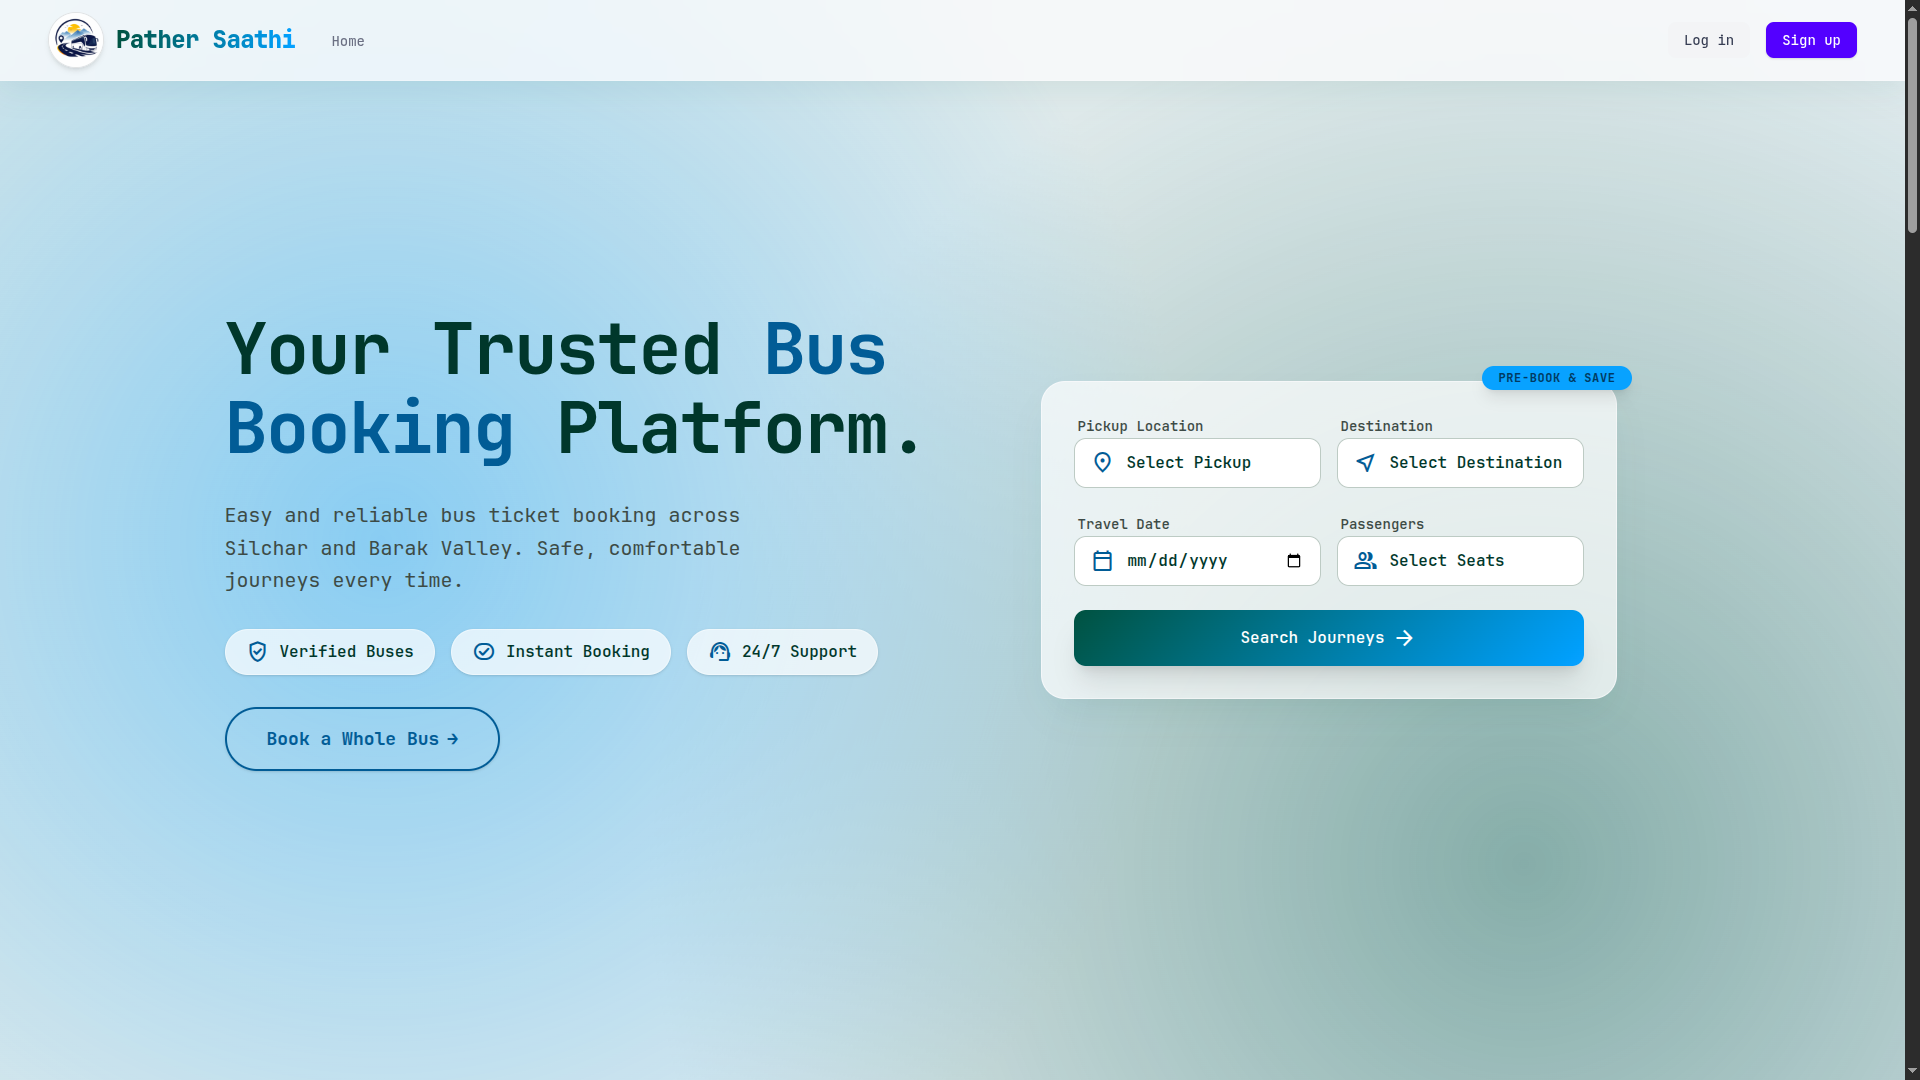
\includegraphics[width=\textwidth]{homepage.png}
    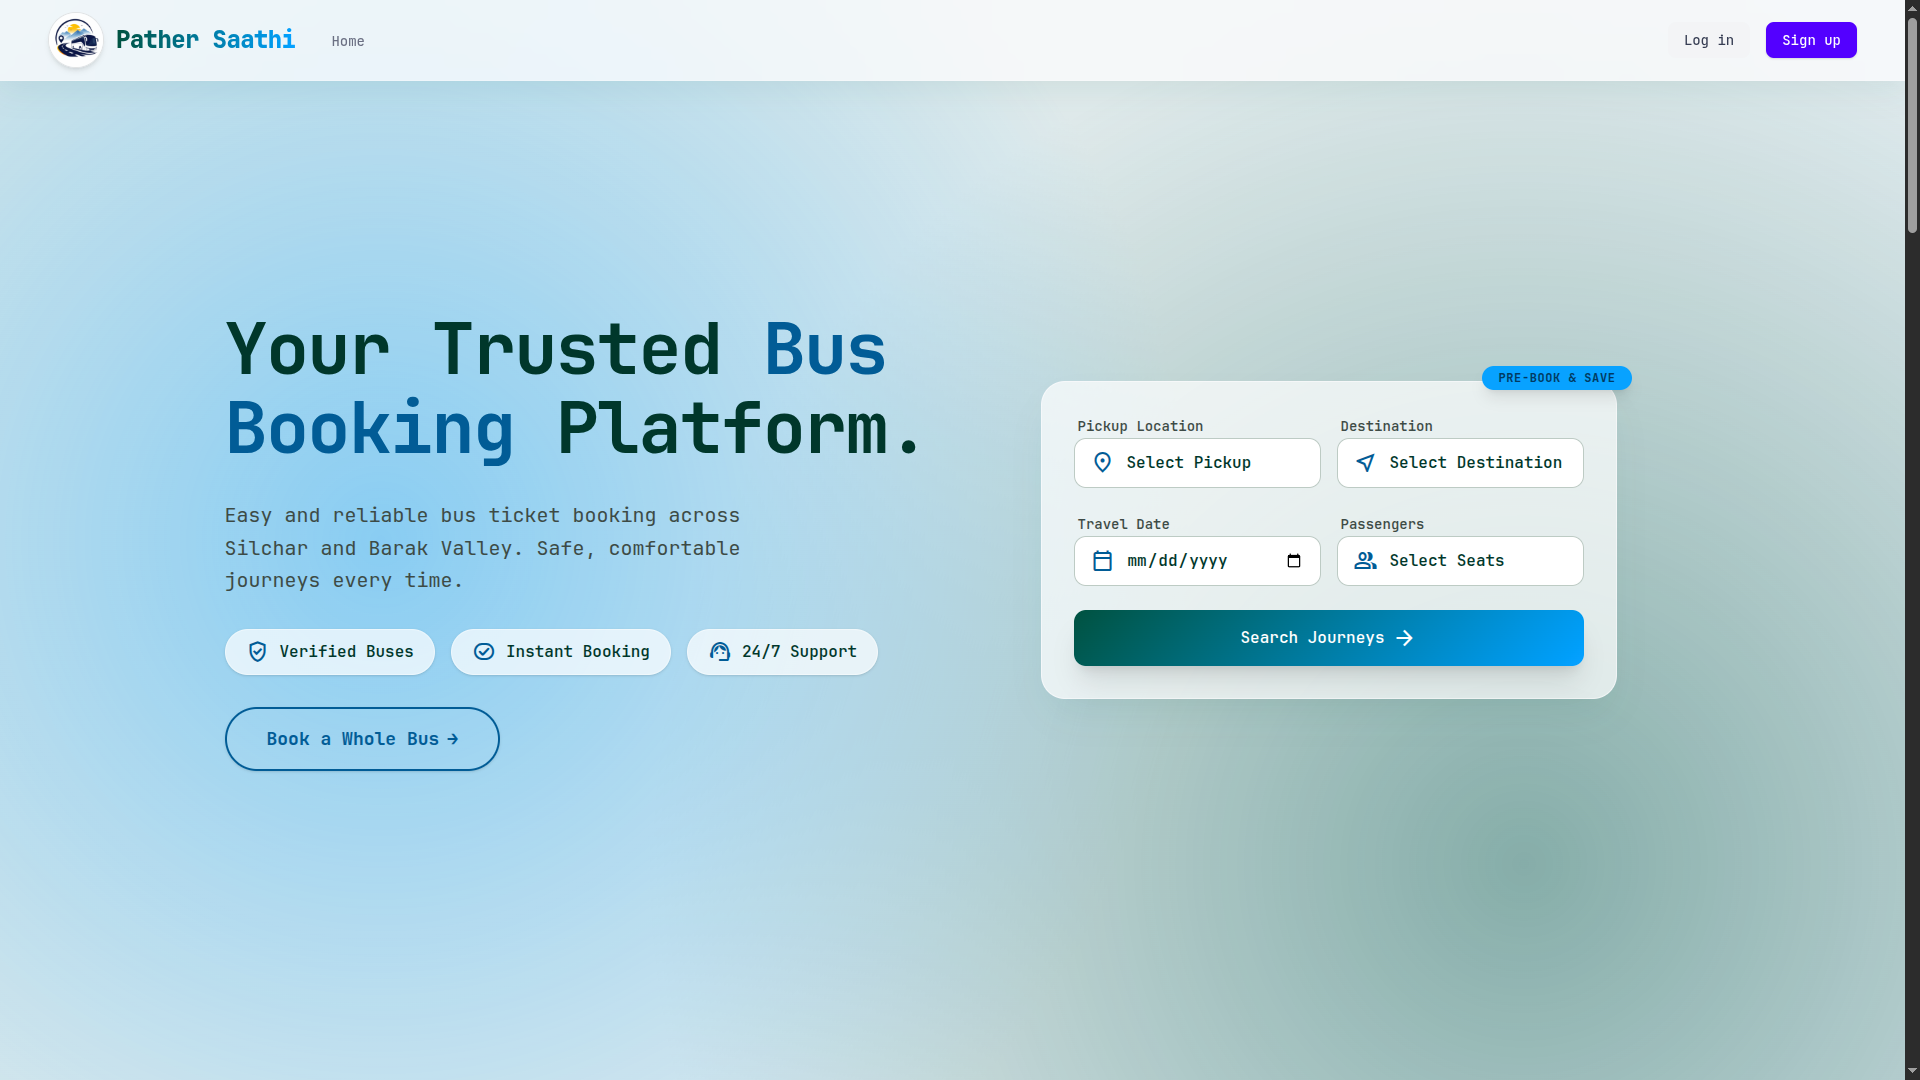
\includegraphics[width=\textwidth]{homepage.png}
}{Pather Saathi Landing Page \& Route Search}{homepage}

\section{Authentication Flow}
The authentication interface provides a seamless, secure login experience. Customers can log in via OTP (if configured) or standard credentials, while operators are directed to a role-gated portal.

\screenshot{
    % \includegraphics[width=\textwidth]{login.png}
    \includegraphics[width=\textwidth]{login.png}
}{Secure Authentication Portal}{login}

\section{Customer Booking Interface}
The core customer workflow isolates the route discovery and seat selection process. The interface explicitly highlights seat availability, vehicle type, and estimated departure times, culminating in the WhatsApp deep-link generation.

\screenshot{
    % \includegraphics[width=\textwidth]{booking.png}
    \includegraphics[width=\textwidth]{booking.png}
}{Seat Selection and Booking Confirmation}{booking}

\section{Operator Dashboard}
The Operator Dashboard acts as a command centre. The interface is data-dense but logically separated, allowing operators to instantly approve or reject pending requests, monitor revenue, and manage their fleet.

\screenshot{
    % \includegraphics[width=\textwidth]{dashboard.png}
    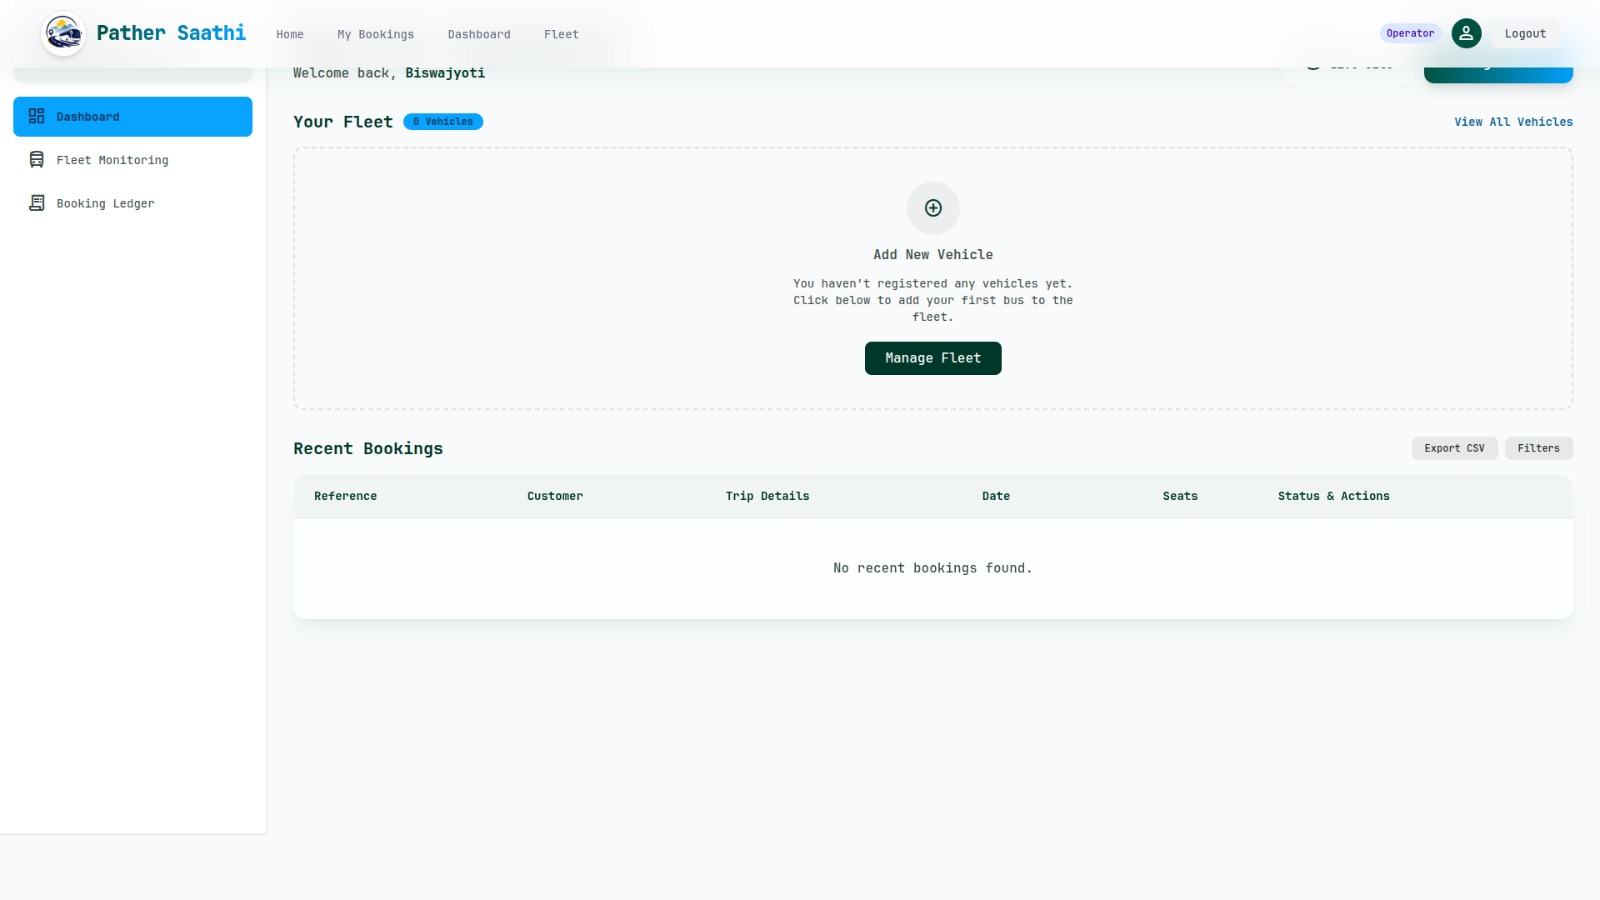
\includegraphics[width=\textwidth]{operator-dashboard.png}
}{Operator Real-Time Dashboard}{dashboard}

\section{Profile \& Configuration}
Both customers and operators have access to configuration panels to manage their metadata, vehicle registrations (for operators), and past booking histories.

\screenshot{
    % \includegraphics[width=\textwidth]{profile.png}
    \includegraphics[width=\textwidth]{profile.png}
}{User Profile and Configuration Management}{profile}

% --- CHAPTER 9 ---
\chapter{Experiments and Results}

\section{Adversarial RLS Security Audit}

\textbf{Objective:} To mathematically verify that the database isolation holds under simulated attacks from compromised tenant accounts. \\
\textbf{Method:} Using direct SQL execution, an attempt was made to manipulate the \texttt{bookings} table by updating the status of a booking belonging to a different operator, simulating an authorisation bypass attack.

\begin{table}[H]
    \centering
    \caption{Adversarial Testing Results}
    \renewcommand{\arraystretch}{1.5}
    \begin{tabularx}{\textwidth}{l X X X}
    \toprule
    \rowcolor{brandteal}
    \textcolor{white}{\textbf{Test}} & \textcolor{white}{\textbf{Scenario}} & \textcolor{white}{\textbf{Result}} & \textcolor{white}{\textbf{Action Taken}} \\
    \midrule
    \rowcolor{lightgray}
    RLS Bypass & Update booking ID belonging to Operator B using Operator A's JWT. & Failed (0 rows affected). RLS successfully blocked the query. & None required. Security validated. \\
    Recursion Bug & Attempted to query user roles recursively in a policy. & Infinite Recursion Error encountered. & Implemented SECURITY DEFINER helper. \\
    \bottomrule
    \end{tabularx}
\end{table}

During the audit, an infinite recursion bug was discovered when complex policies attempted to join back onto the \texttt{users} table. The resolution required implementing a \texttt{SECURITY DEFINER} helper function:

\begin{lstlisting}[language=SQL, caption={SECURITY DEFINER Helper Function}]
CREATE OR REPLACE FUNCTION 
public.user_owns_booking(booking_uuid UUID)
RETURNS BOOLEAN
LANGUAGE sql STABLE SECURITY DEFINER
SET search_path = public
AS $$
  SELECT EXISTS (
    SELECT 1 FROM bookings
    WHERE id = booking_uuid
    AND customer_id = auth.uid()
  );
$$;
\end{lstlisting}

\section{Validation Summary}
The culmination of these experimental testing phases confirmed the operational readiness of the platform. Adversarial security audits proved the RLS layer to be mathematically resilient against privilege escalation and tenant data leakage. Distributed load testing validated the edge-based rate limiting architecture, ensuring protection against automated abuse. Finally, the end-to-end booking flow and build integrity metrics confirmed that the core business logic performs reliably under real-world constraints without producing runtime errors or TypeScript violations.

\section{Rate Limiting Architecture Validation}
\textbf{Hypothesis:} An in-memory \texttt{Map} will successfully rate-limit API abuse on a local development server, but will fail in a distributed serverless environment.\\
\textbf{Method:} Executed a high-concurrency brute-force attack against the authentication endpoint using a load testing script after deploying to Vercel.\\
\textbf{Finding:} Vercel's ephemeral edge instances spun up isolated environments, bypassing the in-memory Map entirely.\\
\textbf{Resolution:} Architected a distributed rate-limiting solution using Upstash Redis. The subsequent load test successfully throttled the attack globally across all edge nodes.

\section{End-to-End Booking Flow Validation}
\begin{table}[H]
    \centering
    \caption{E2E Flow Validation}
    \renewcommand{\arraystretch}{1.5}
    \begin{tabularx}{\textwidth}{l X X}
    \toprule
    \rowcolor{brandteal}
    \textcolor{white}{\textbf{Step}} & \textcolor{white}{\textbf{Action}} & \textcolor{white}{\textbf{Result}} \\
    \midrule
    \rowcolor{lightgray}
    1 & Customer initiates booking for 2 seats. & Transaction atomic lock acquired. \\
    2 & Database validates availability. & Seats decremented, status set to pending. \\
    \rowcolor{lightgray}
    3 & WhatsApp deep-link triggered. & Native app opens with pre-filled message. \\
    4 & Operator approves via dashboard. & Status updated to approved, confirmation visible. \\
    \bottomrule
    \end{tabularx}
\end{table}

\section{Build Integrity Results}
\begin{table}[H]
    \centering
    \caption{Build Integrity Metrics}
    \renewcommand{\arraystretch}{1.5}
    \begin{tabularx}{\textwidth}{X X}
    \toprule
    \rowcolor{brandteal}
    \textcolor{white}{\textbf{Metric}} & \textcolor{white}{\textbf{Result}} \\
    \midrule
    \rowcolor{lightgray}
    TypeScript Type Errors & 0 \\
    ESLint Warnings/Errors & 0 \\
    \rowcolor{lightgray}
    Vercel Production Build Exit Code & 0 (Success) \\
    Average Turbopack Build Time & $\sim$3.0 seconds \\
    \bottomrule
    \end{tabularx}
\end{table}

\section{Production Readiness Assessment}
\begin{keyfinding}[title=\textbf{Production Status: MVP Ready}]
The Pather Saathi platform has successfully passed all critical adversarial testing, build verification, and end-to-end integration flows. The core MVP features (discovery, booking, operator dashboard, and WhatsApp integration) are functionally complete and mathematically secure under simulated load. The system is currently staged for pilot deployment with select operators in the Barak Valley region. Features such as formal payment gateways and native app wrappers have been intentionally deferred to the future scope to ensure the absolute stability of the core concurrency engine.
\end{keyfinding}

% --- CHAPTER 10 ---
\chapter{Challenges Faced}

\section{RLS Infinite Recursion Bug}
The most profound database engineering challenge occurred during the implementation of complex Row Level Security (RLS) policies. To verify if a user had the authority to view a specific booking, the policy attempted to join the \texttt{bookings} table with the \texttt{users} table to check the user's role. However, the \texttt{users} table itself had an RLS policy that referenced the \texttt{bookings} table, resulting in an infinite recursive loop that crashed the PostgreSQL instance during testing. The resolution required extensive architectural redesign, ultimately leveraging \texttt{SECURITY DEFINER} functions to bypass the policy evaluation loop while maintaining strict row-level isolation. This lesson reinforced the importance of flat policy evaluation in multi-tenant systems.

\begin{lessonslearned}
Multi-tenant security policies must be strictly non-recursive. Utilizing \texttt{SECURITY DEFINER} functions to bypass policy evaluation loops is mandatory for complex RBAC schemas.
\end{lessonslearned}

\section{In-Memory Rate Limiting on Vercel Serverless}
A significant infrastructural challenge arose from a misunderstanding of serverless deployment models. The initial security implementation utilised a standard JavaScript \texttt{Map} object to track request frequencies and enforce rate limits against API endpoints. While this functioned perfectly locally, it failed entirely upon deployment. Vercel provisions isolated, ephemeral serverless instances for concurrent requests, meaning memory is not shared. A brute-force attacker could bypass the limit by distributing requests. This required an immediate architectural pivot, integrating Upstash Redis to provide a centralised, distributed memory store, teaching the team critical lessons about stateless architecture design.

\begin{lessonslearned}
Serverless functions execute in isolated, ephemeral environments. State cannot be reliably shared in memory across requests; a distributed cache like Upstash Redis is non-negotiable for global rate limiting.
\end{lessonslearned}

\section{Environment Variable Management Across Local and Production}
Managing the environmental disparity between the local Supabase development container and the Vercel serverless production environment proved to be a persistent operational challenge. Coordinating environment variables, specifically the cryptographic JWT secrets and database connection strings, required meticulous manual synchronisation. Because the AI-augmented workflow generated highly complex database migrations locally, deploying these changes required strict, manual operational cadence using the \texttt{supabase db push --linked} command to prevent catastrophic schema mismatches. The team had to establish strict runbooks for deployment to manage this operational overhead.

\section{AI-Generated Code Quality Control}
While the AI-augmented methodology provided massive gains in development velocity, the raw quality of the generated code presented continuous challenges. Early iterations suffered from inconsistent naming conventions and subtle logical flaws. Initial generated iterations of the authentication actions contained mass assignment vulnerabilities. These issues necessitated the implementation of the secondary adversarial review passes. By forcing different AI models to critique the code generated by the primary agent, the human team was able to identify and patch vulnerabilities before deployment. This highlighted that AI is an execution multiplier, not a replacement for architectural oversight.

\section{Performance on Low-End Android Devices}
During initial field testing, the platform exhibited sluggish performance on entry-level Android devices commonly used in Barak Valley. The React hydration process was excessively long due to large client-side JavaScript bundles, causing noticeable input lag on the booking interface. The engineering team resolved this by aggressively refactoring the component tree to utilise React Server Components (RSC), drastically reducing the JavaScript payload sent to the client and resulting in near-instantaneous interaction times on low-end devices. This reinforced the necessity of hardware-constrained testing paradigms.

\section{Project Scope Management}
Given the ease of feature implementation provided by AI orchestration, the team faced intense pressure regarding scope creep. It was highly tempting to continuously add features such as integrated payment gateways, live GPS vehicle tracking, and complex analytics dashboards. However, managing this scope was critical to delivering a polished MVP. The team had to ruthlessly prioritise features that directly addressed the core problem of double bookings and discovery, intentionally delaying secondary features to the future scope to ensure the core platform was perfectly stable and secure prior to the presentation deadline.

% --- CHAPTER 10 ---
\chapter{Future Scope}

\section{Construction Vehicle Booking (Phase 2)}
The initial architecture of Pather Saathi has been intentionally designed to be extensible beyond passenger transit. The immediate future scope involves expanding the platform to encompass heavy construction and logistics vehicle chartering (e.g., excavators, dump trucks). The database schema already supports varying vehicle types, requiring only frontend modifications to accommodate payload capacities and hourly rate structures rather than seat-based pricing.

\section{Online Payment Integration --- Razorpay}
Currently, the platform relies on physical cash exchanges or direct UPI transfers negotiated via WhatsApp. Integrating a formal payment gateway, such as Razorpay, will allow operators to mandate partial deposits to secure bookings, drastically reducing the rate of customer no-shows. This integration will be built directly into the Next.js Server Actions to ensure cryptographic verification of payment webhooks.

\section{Seat Selection Interface}
To further reduce friction, a visual seat selection interface will be implemented for scheduled bus routes. This will allow customers to select specific seat numbers during the booking flow, dynamically updating the database and locking the selected seats via atomic PostgreSQL transactions to prevent concurrent selections.

\section{Email and SMS Notifications}
While WhatsApp is the primary communication layer, implementing fallback notification systems via SMS (using Twilio or Msg91) and email (using Resend or Cloudflare Email Service) will ensure critical booking confirmations and cancellations reach users who may experience intermittent internet connectivity.

\section{Native Mobile Application}
Although the Progressive Web App (PWA) provides excellent functionality, wrapping the application in a lightweight native Android shell (using React Native or Capacitor) would allow for push notifications and deeper hardware integration, further cementing the platform's utility for daily commuters.

\section{Multi-District Operator Expansion}
Once the operational model is fully validated in Barak Valley, the platform architecture allows for seamless scaling to other districts within Assam and Northeast India. The multi-tenant database design ensures that scaling operator accounts requires zero architectural modifications.

\section{Analytics Dashboard for Operators}
Providing operators with predictive analytics based on historical booking data will enable them to dynamically adjust pricing and schedule frequencies based on anticipated demand, transforming their operational efficiency from reactive to proactive.

\section{Formalised AI Development Methodology as a Reusable Framework}
Beyond the software product, the AI-augmented development methodology pioneered during this project has significant future potential. Formalising this workflow into a reusable, documented framework will allow other resource-constrained engineering teams to safely and rapidly architect enterprise-grade software solutions using Model Context Protocol orchestration.

% --- CHAPTER 11 ---
\chapter{Conclusion}

Pather Saathi successfully demonstrates the profound impact that highly localised, context-aware digital platforms can have on underserved regional economies. By architecting a robust, cost-efficient fleet booking system tailored explicitly for the socioeconomic and technological realities of Barak Valley, this project effectively bridges a critical infrastructural gap. The decision to bypass complex, proprietary messaging systems in favour of integrating directly with the universally adopted WhatsApp ecosystem proved to be a decisive factor in reducing user friction and ensuring operational viability for local fleet owners. The platform completely eliminates the pervasive issue of double bookings by replacing analogue ledgers with a highly concurrent, mathematically secure cloud database.

A paramount achievement of this project is the rigorous application of enterprise-grade security within a serverless architecture. By treating the database as a zero-trust environment and enforcing strict Row Level Security (RLS) and Role-Based Access Control (RBAC) at the lowest architectural level, the platform guarantees absolute data isolation between competing fleet operators. The successful mitigation of complex architectural vulnerabilities, such as infinite recursion bugs in policy definitions and distributed rate-limiting failures on ephemeral edge networks, underscores the engineering depth applied to the project. The final deployed product is not merely a prototype, but a production-hardened system capable of securely scaling to meet regional demand.

Furthermore, this project makes a significant contribution to the evolving discourse on modern software engineering methodologies. It serves as a practical, empirical validation of AI-augmented development orchestration. By leveraging multi-model AI agents via the Model Context Protocol (MCP), the team operated at a level of architectural sophistication and development velocity traditionally reserved for much larger, highly resourced enterprise teams. Pather Saathi stands as a testament to the future of software engineering: where human engineers act as strategic orchestrators and security auditors, directing AI capabilities to construct complex, impactful, and secure solutions for local communities.

\section{Project Impact Assessment}
The deployment of Pather Saathi fundamentally transforms the operational paradigm for regional fleet owners. By providing an enterprise-grade digital infrastructure at minimal cost, the platform democratises access to sophisticated fleet management previously gated by prohibitive licensing fees. For the citizens of Barak Valley, it converts a frustrating, opaque booking process into a transparent, secure, and instant digital experience. Ultimately, the project proves that context-aware software engineering, combined with AI-augmented workflows, can rapidly and effectively solve critical socio-economic inefficiencies in Tier-3 demographics.

\renewcommand{\bibname}{References}
\addcontentsline{toc}{chapter}{References}
\nocite{*}
\bibliographystyle{ieeetr}
\bibliography{references}

\end{document}
